% =============================================
% LOF & centroid 補足説明追加版(リファイン)
% =============================================

\documentclass[a4j,dvipdfmx]{jsarticle}
\usepackage{graphicx}
\usepackage{amsmath}
\usepackage{url}
\usepackage{algorithm}
\usepackage{algorithmic}
\usepackage{booktabs}
\usepackage{float} % 図の位置制御用

\floatname{algorithm}{アルゴリズム}

% 浮動体のパラメータ調整
\renewcommand{\topfraction}{0.85}
\renewcommand{\bottomfraction}{0.85}
\renewcommand{\textfraction}{0.15}
\renewcommand{\floatpagefraction}{0.7}

\title{二次元データに対する k-means クラスタリングと Local Outlier Factor の C\# 実装}
\author{大阪大学 工学部 電子情報学科 3 年\\情報システム工学コース\\08D23091\,辻\,孝弥}
\date{\today}

%--------------------------------------------------
\begin{document}
\maketitle
\tableofcontents
\newpage

%--------------------------------------------------
\begin{abstract}
最大 200 点の二次元データを入力とし,Local Outlier Factor (LOF) で外れ値を検出した後に k-means クラスタリングを連続実行する C\# プログラムを作成した。本稿ではその実装要点と実験結果を報告する。加えて,入出力仕様,実行ログの要約,将来の改良方針を示す。
\end{abstract}

%--------------------------------------------------
\section{背景と目的}
外れ値検出とクラスタリングはデータ解析の基盤技術であり,相互に強く影響しあう。本プログラムは,まず LOF で外れ値を排除し,その後 k-means を適用することでクラスタリング結果の安定性を高めることを目的とする。

%--------------------------------------------------
\section{手法}
\subsection{処理フロー}
\begin{description}
  \item[入力] 二次元座標を格納した CSV ファイル(書式:\texttt{x,y})。
  \item[処理手順]
    \begin{enumerate}
      \item CSV の読み込み
      \item LOF の計算(近傍数 $k=10$)
      \item LOF 値が 1.2 を超えた点を外れ値としてフラグ付け
      \item k-means クラスタリング(クラスタ数はコマンドライン引数,既定値 3)
      \item 結果を CSV に出力
    \end{enumerate}
  \item[出力] \texttt{x, y, cluster\_id, is\_outlier}
\end{description}

\subsection{Local Outlier Factor (LOF)}
点 $A$ の LOF は次式で定義される:
\begin{equation}
  \operatorname{LOF}_k(A)=\frac{\displaystyle\frac{1}{|N_k(A)|}\sum_{B\in N_k(A)} \operatorname{lrd}_k(B)}{\operatorname{lrd}_k(A)}\, ,
  \label{eq:lof}
\end{equation}
ここで $N_k(A)$ は $A$ の $k$ 近傍集合,$|N_k(A)|=k$,$\operatorname{lrd}_k(\cdot)$ は局所到達可能密度 (Local Reachability Density) である。

\subsection{k-means クラスタリング}
初期重心はランダムに選択し,ユークリッド距離で各点を割り当て,重心を再計算する。この更新を
\[
  \max_{j} \bigl\| \mathbf{c}_{j}^{(t+1)}-\mathbf{c}_{j}^{(t)} \bigr\| < 10^{-8}
\]
が成り立つか,または 1000 反復に到達するまで繰り返す。$\mathbf{c}_{j}^{(t)}$ は時刻 $t$ におけるクラスタ $j$ の重心であり,実装では配列 \texttt{centroid[j,*]} に対応する。\textbf{外れ値フラグが立った点は重心計算に含めない。}

%--------------------------------------------------
\section{実装要点 (C\#)}
\begin{itemize}
  \item 2 次元データは \texttt{double[,]} 配列で保持し,最大 200 行を想定。
  \item LOF と k-means は同一ソースファイルに実装し,外部ライブラリは不使用。
  \item 外れ値を除外して重心を再計算するコード断片をアルゴリズム~\ref{lst:centroid} に示す。
\end{itemize}

\begin{algorithm}[tbp]
\caption{外れ値除外付き重心計算(抜粋)}
\label{lst:centroid}
\begin{algorithmic}[1]
\FOR{$i \gets 0$ \TO $N-1$}
  \IF{$label[i]==k$ \AND $is\_outlier[i]==\text{false}$}
    \STATE $\text{sum}_x \mathrel{+}= data[i,0]$;
    \STATE $\text{sum}_y \mathrel{+}= data[i,1]$;
    \STATE $\text{count} \mathrel{+}=1$;
  \ENDIF
\ENDFOR
\end{algorithmic}
\end{algorithm}

%--------------------------------------------------
\section{実験設定}
\subsection{データセット}
5 種の人工データセット(各 200 点)を使用した:\texttt{moon},\texttt{crater},\texttt{square},\texttt{three\_island},\texttt{two\_island}。

\subsection{パラメータ}
LOF の近傍数は $k=10$,閾値は 1.2。k-means のクラスタ数は 3(任意の正の数: コマンドライン引数で指定)とし,収束判定の上限を 1000 反復に設定した。

%--------------------------------------------------
\section{結果}
\subsection{外れ値検出(moon データセット)}
式~\eqref{eq:lof} に基づき LOF を計算した結果,値が 1.2 を超えた点は 7 つであった(表~\ref{tab:outliers})。

\begin{table}[tbp]
  \centering
  \caption{外れ値一覧(LOF $>1.2$)}
  \label{tab:outliers}
  \begin{tabular}{ccc}
    \toprule
    No. & 座標 $(x,y)$ & LOF 値 \\
    \midrule
    1 & (0.2082, 0.9957) & 1.3159 \\
    2 & (0.1641, 1.0172) & 1.2992 \\
    3 & (0.3043, 1.0289) & 1.2795 \\
    4 & (2.2251, 0.9604) & 1.2248 \\
    5 & (0.2126, 0.9937) & 1.3193 \\
    6 & (3.1527, 1.5360) & 1.2000 \\
    7 & (1.1774, 1.6019) & 1.2411 \\
    \bottomrule
  \end{tabular}
\end{table}

\subsection{k-means の収束状況}
\texttt{moon} データセットでは,初期重心をランダムに設定した結果,13 反復で収束した。各反復で前述の 7 点は重心計算から除外された。

\subsection{可視化結果}
図~\ref{fig:moon-crater}, ~\ref{fig:square-three}, ~\ref{fig:two-island} は人工データセットのクラスタリング結果である。これに関する考察は~\ref{sec:discussion} 節で行う。
\begin{figure}[H]
  \centering
  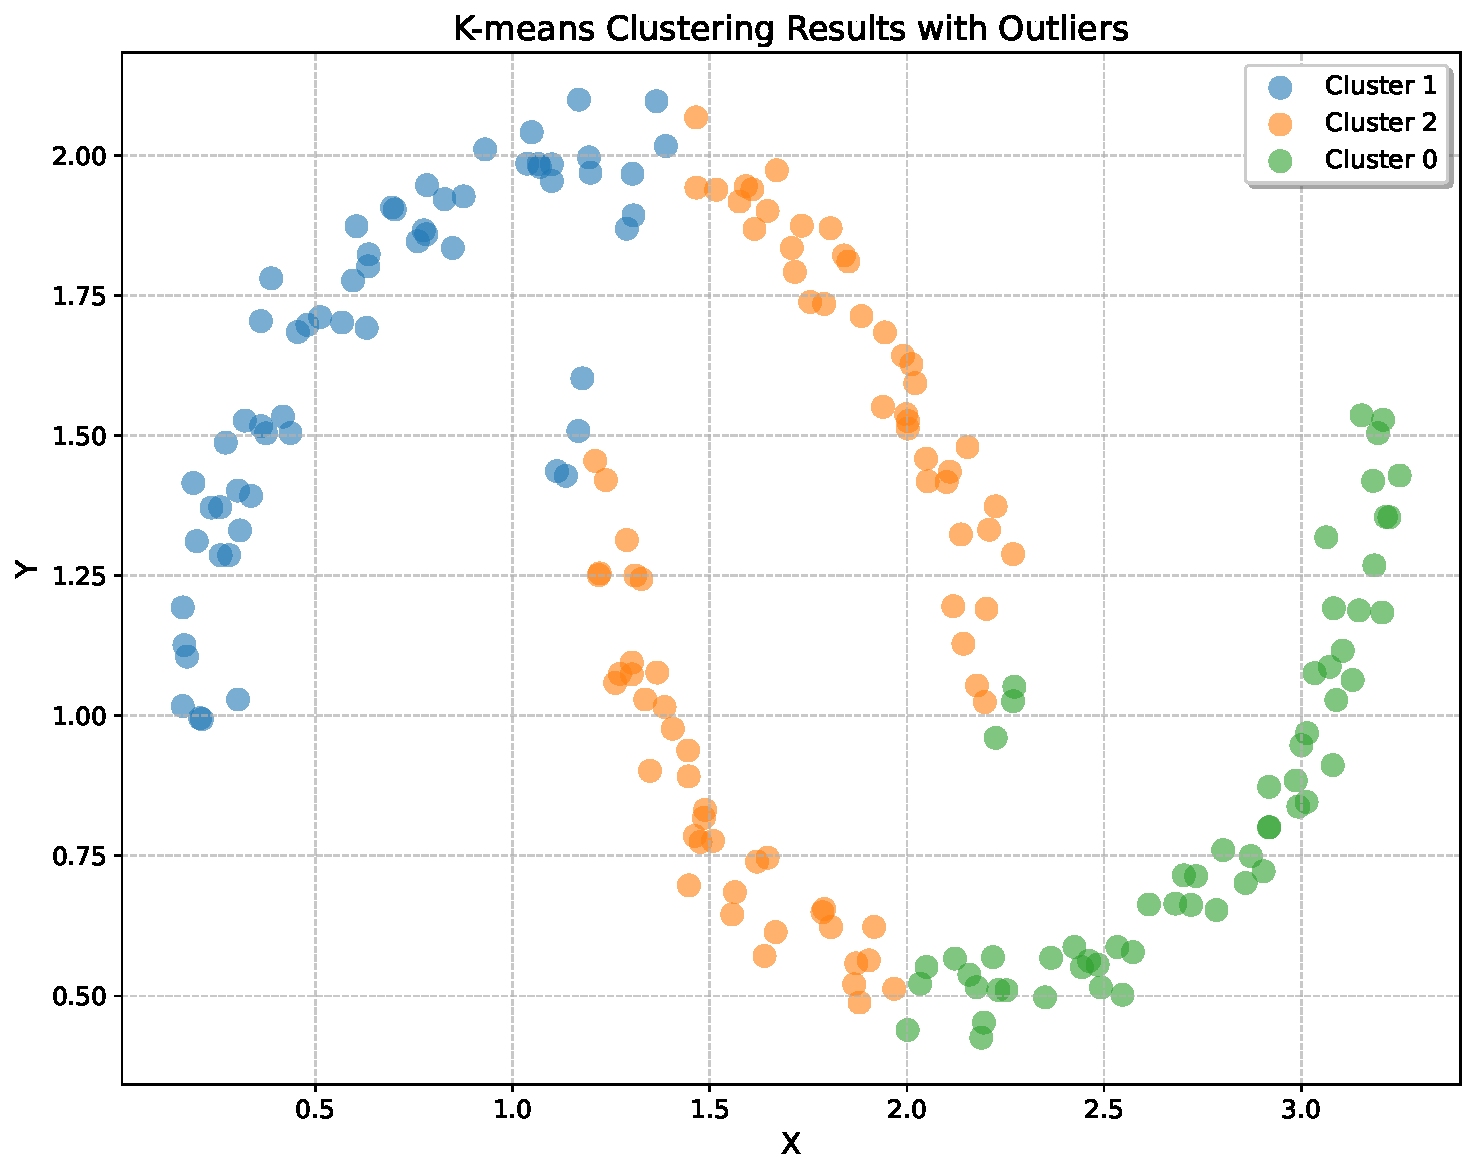
\includegraphics[width=.4\textwidth]{moon_output_plot.pdf}
  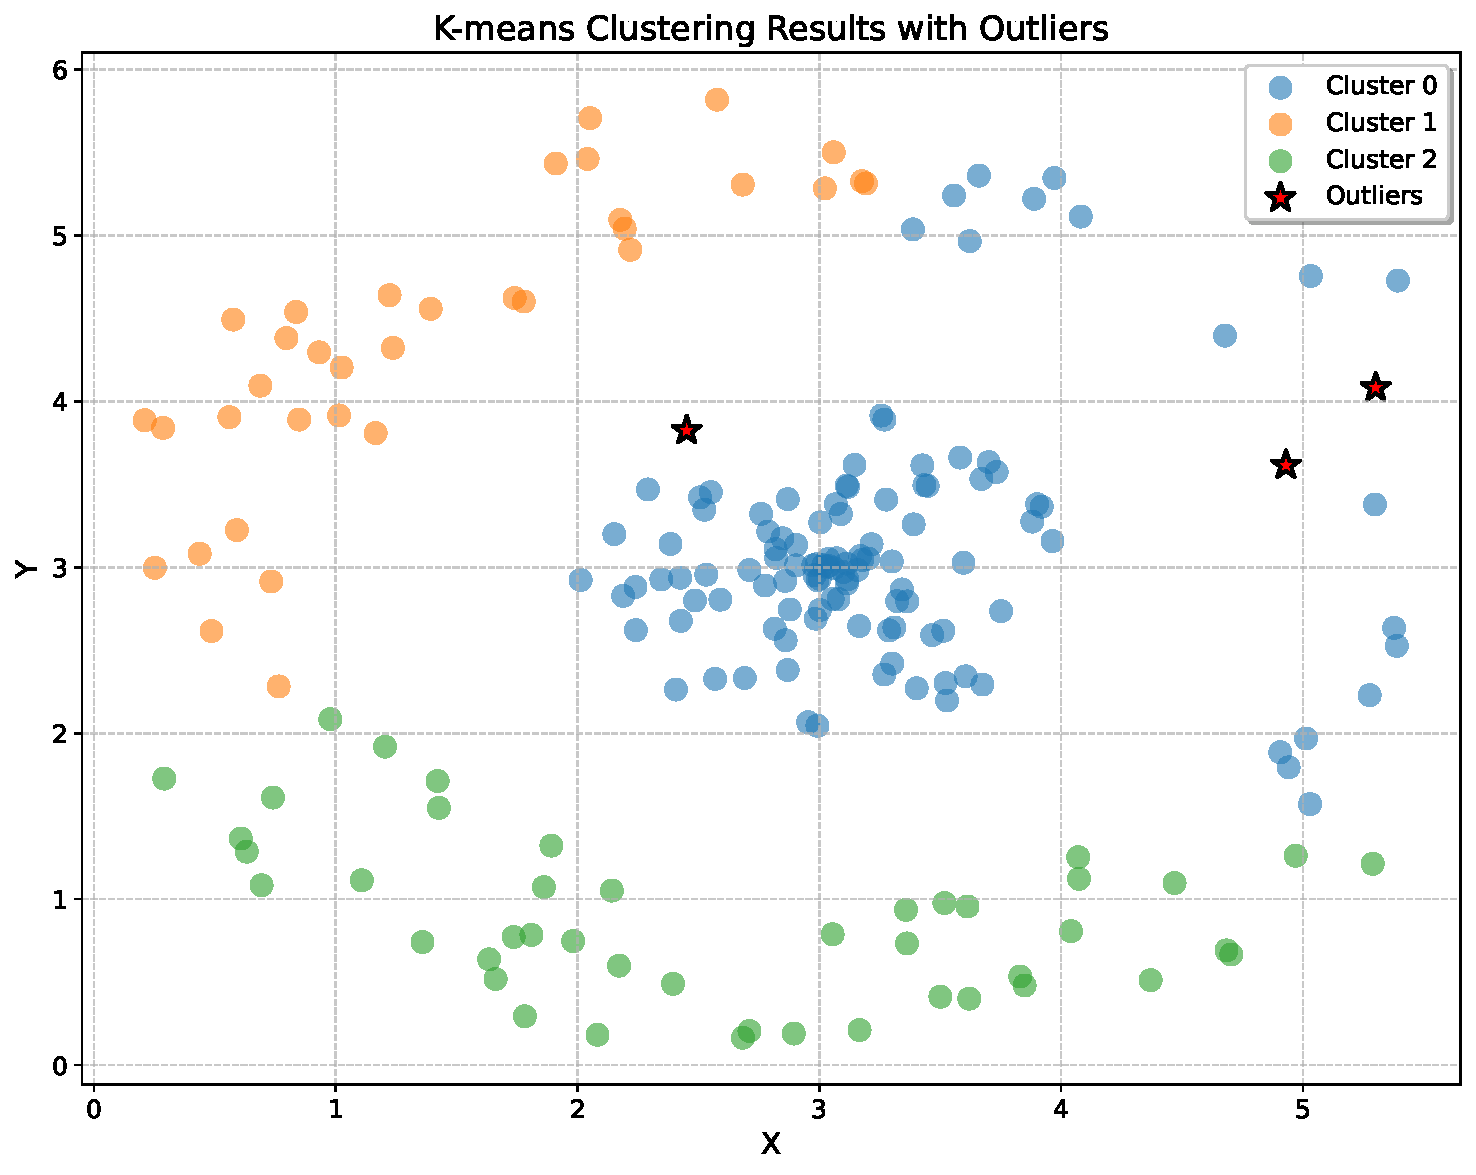
\includegraphics[width=.4\textwidth]{crater_output_plot.pdf}
  \caption{\texttt{moon}(左)と \texttt{crater}(右)のクラスタリング結果}
  \label{fig:moon-crater}
\end{figure}

\begin{figure}[H]
  \centering
  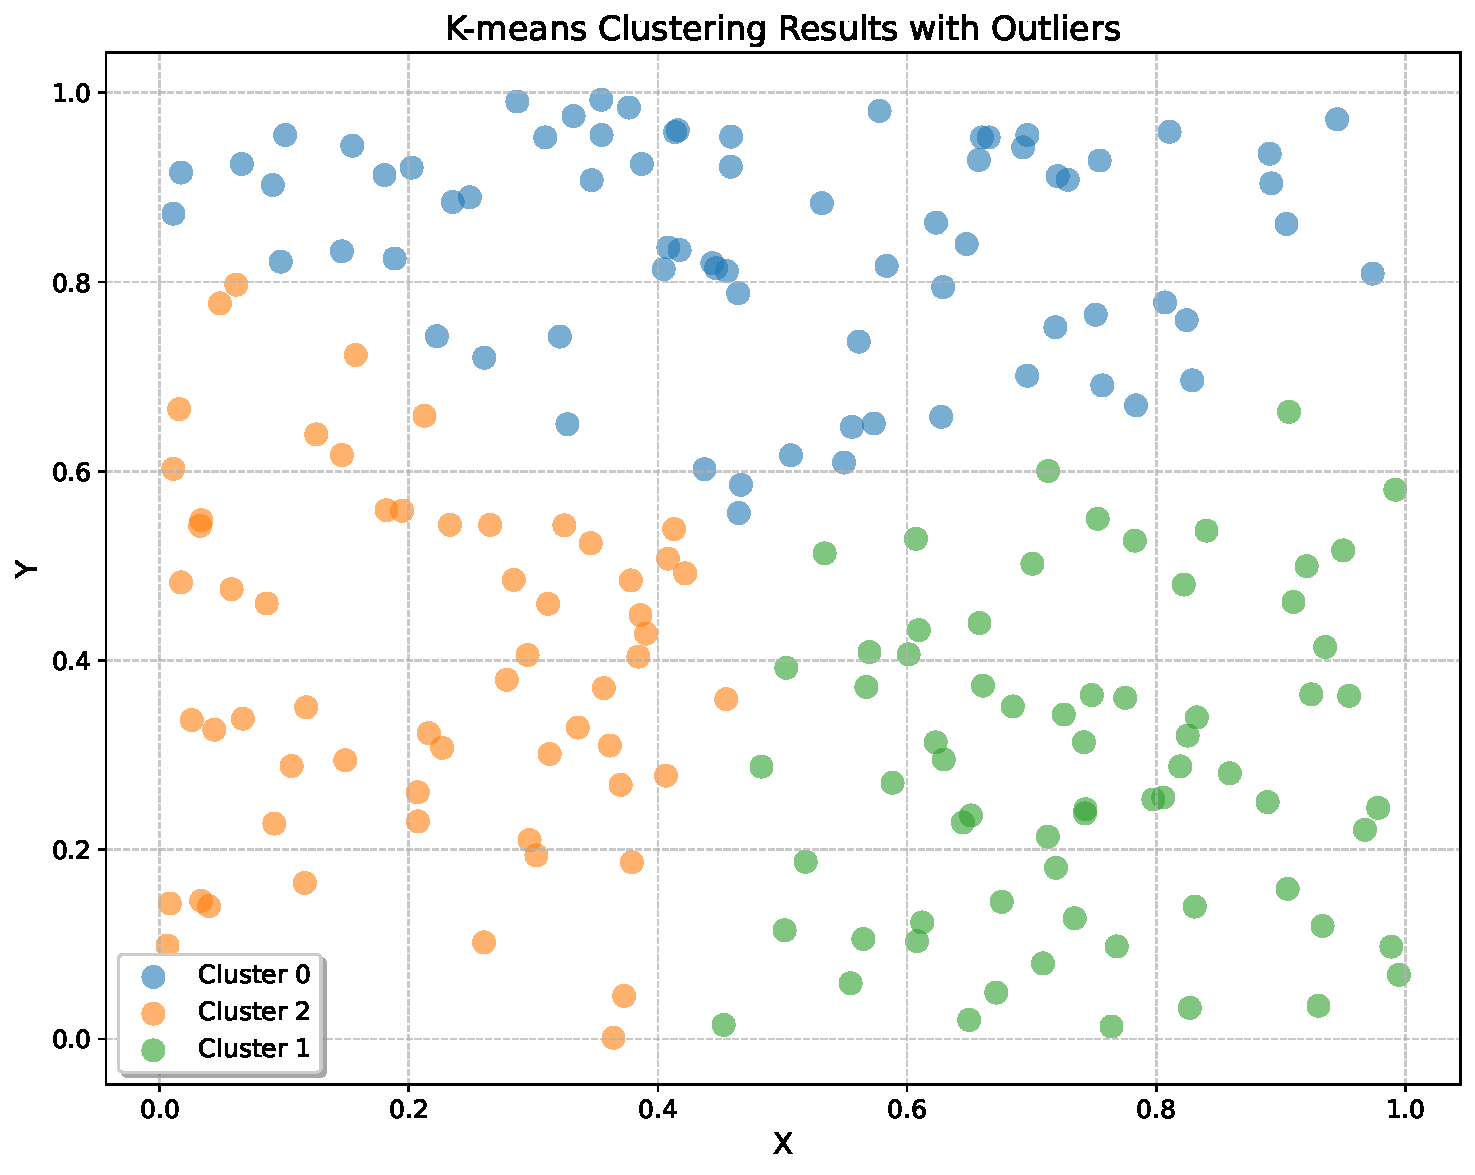
\includegraphics[width=.4\textwidth]{square_output_plot.pdf}
  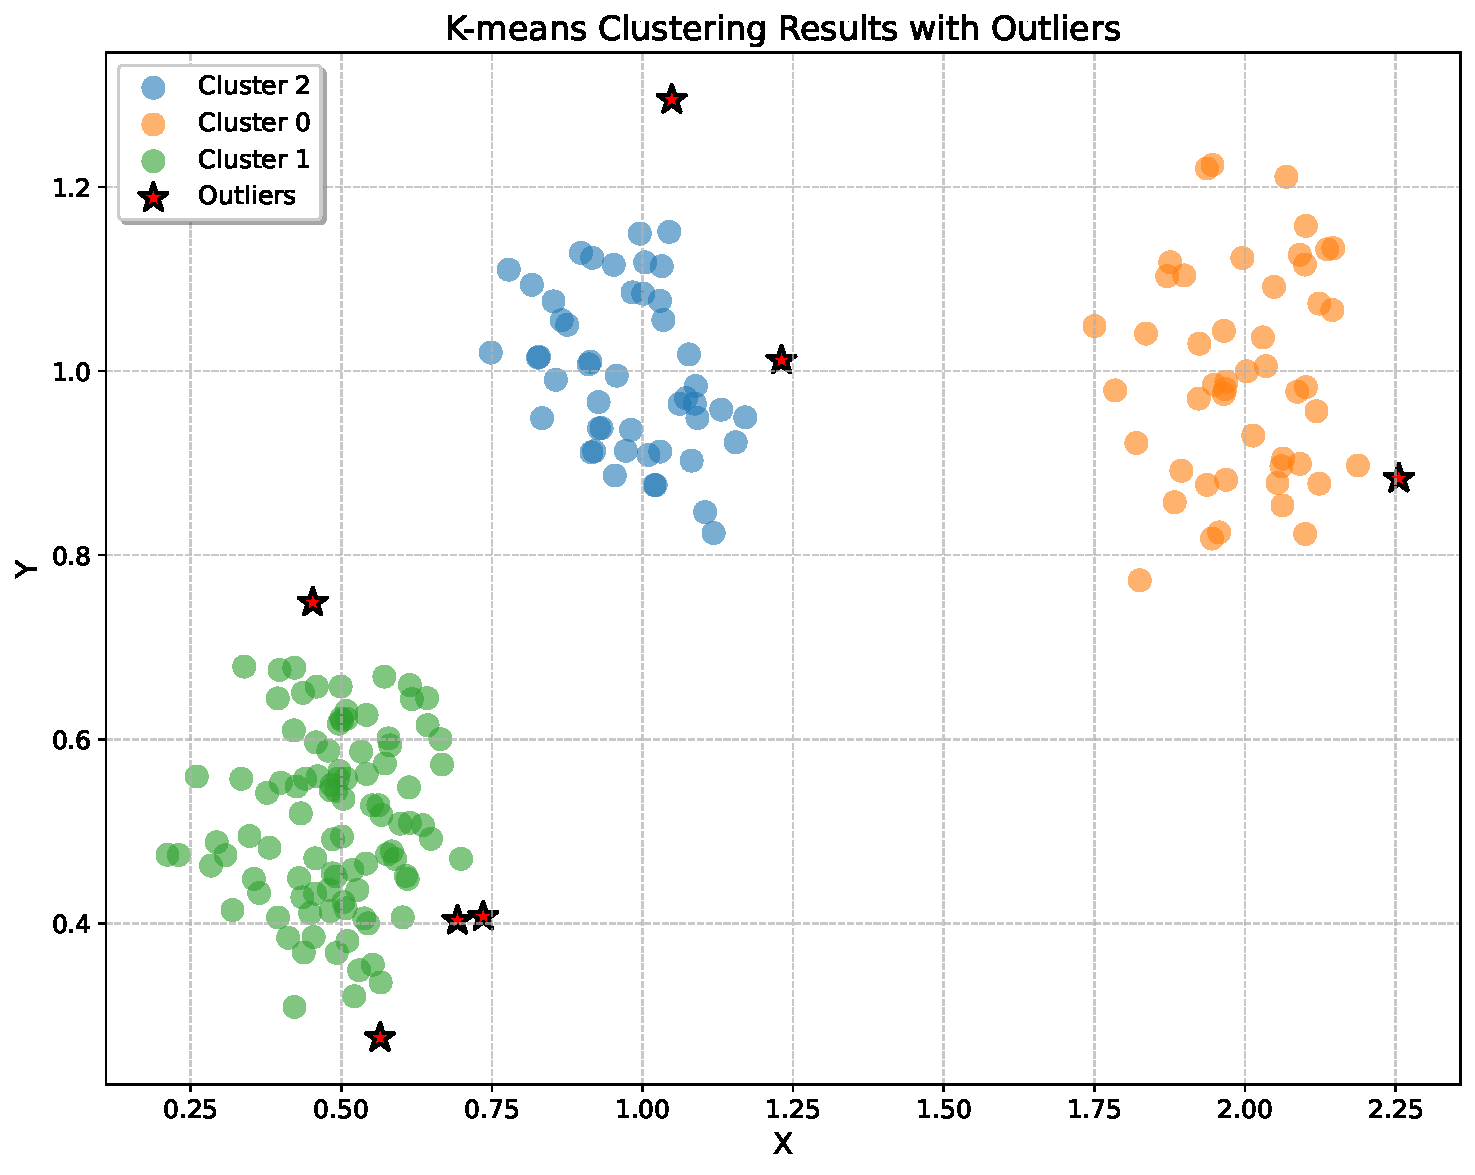
\includegraphics[width=.4\textwidth]{three_island_output_plot.pdf}
  \caption{\texttt{square}(左)と \texttt{three\_island}(右)のクラスタリング結果}
  \label{fig:square-three}
\end{figure}

\begin{figure}[H]
  \centering
  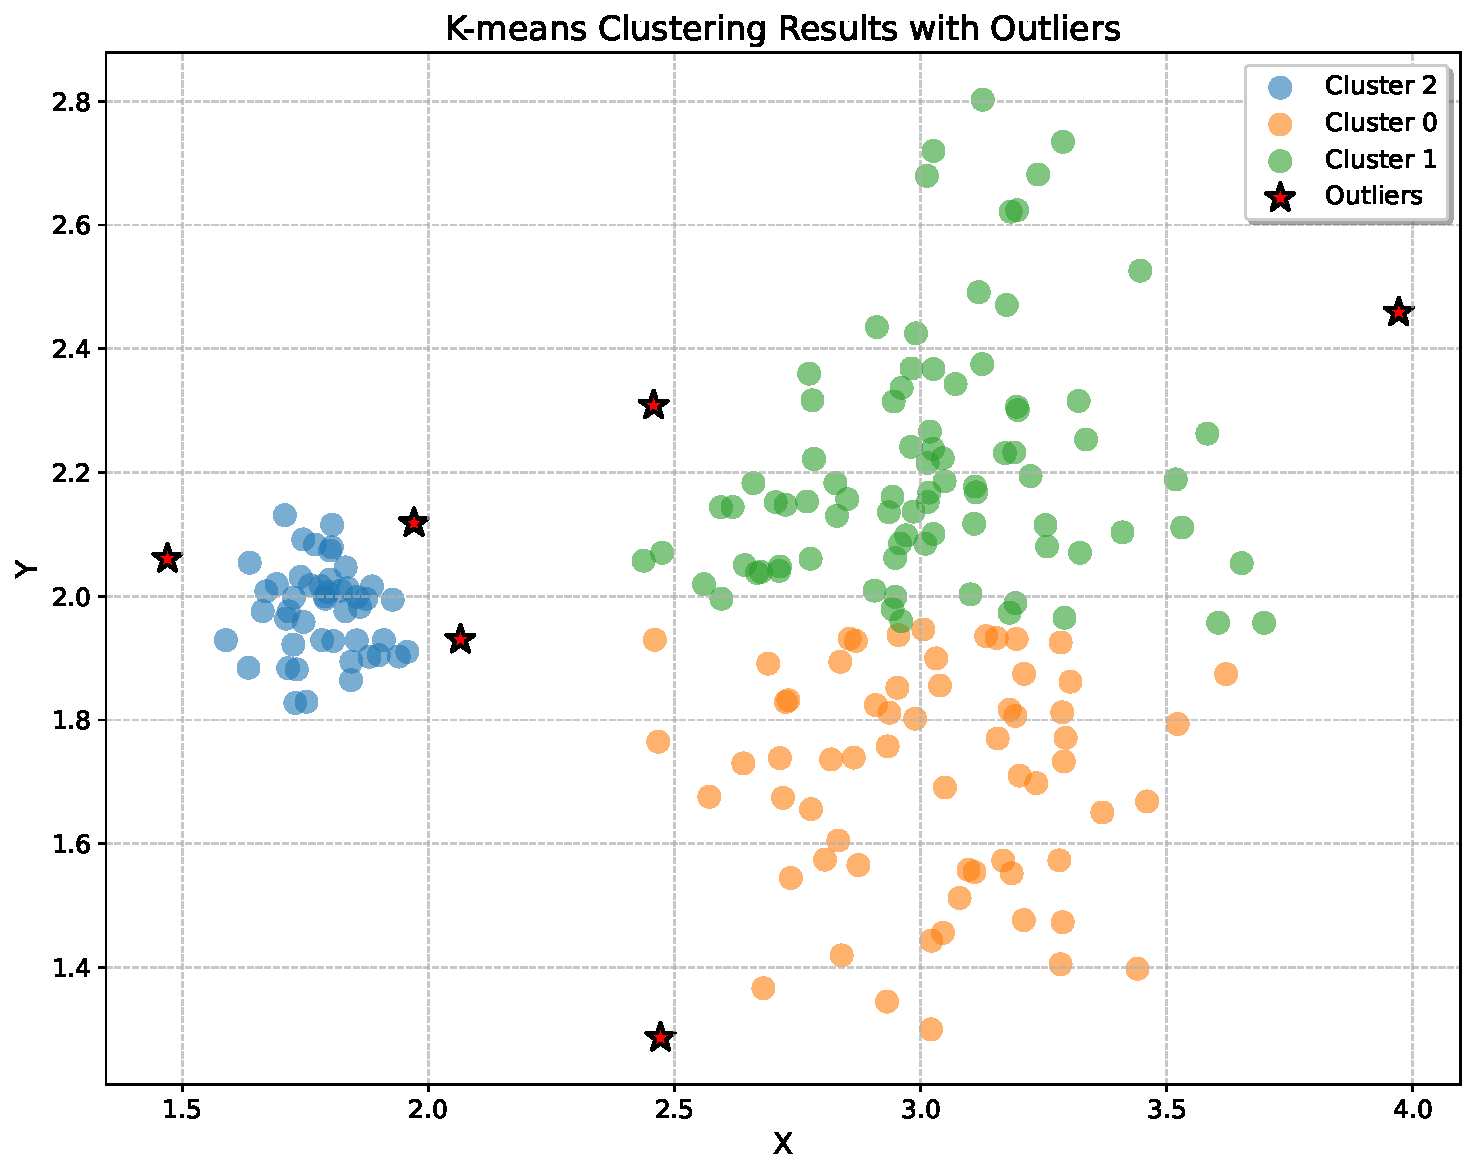
\includegraphics[width=.4\textwidth]{two_island_output_plot.pdf}
  \caption{\texttt{two\_island} データセットのクラスタリング結果}
  \label{fig:two-island}
\end{figure}

%--------------------------------------------------
\section{考察}
\label{sec:discussion}
\subsection{外れ値除去の効果}
\subsubsection{結論}
LOF により外れ値を事前に取り除くことで,各クラスタの重心が極端な点に引きずられず,分割が安定した。特に \texttt{square}, \texttt{three\_island}, \texttt{two\_island} のような単純形状に対しては,再現性の高いクラスタリングが得られた。

\subsubsection{効果の検証}
外れ値除去の有無による差を確認するため,\texttt{two\_island} データに人工外れ値を追加した。外れ値を除外せずにクラスタリングした結果を図~\ref{fig:two-island-with-outlier} に示す。初期重心の選択により 2 通りの分割結果が生じ,いずれも正しいクラスタ構造を再現できていない。

\begin{figure}[H]
  \centering
  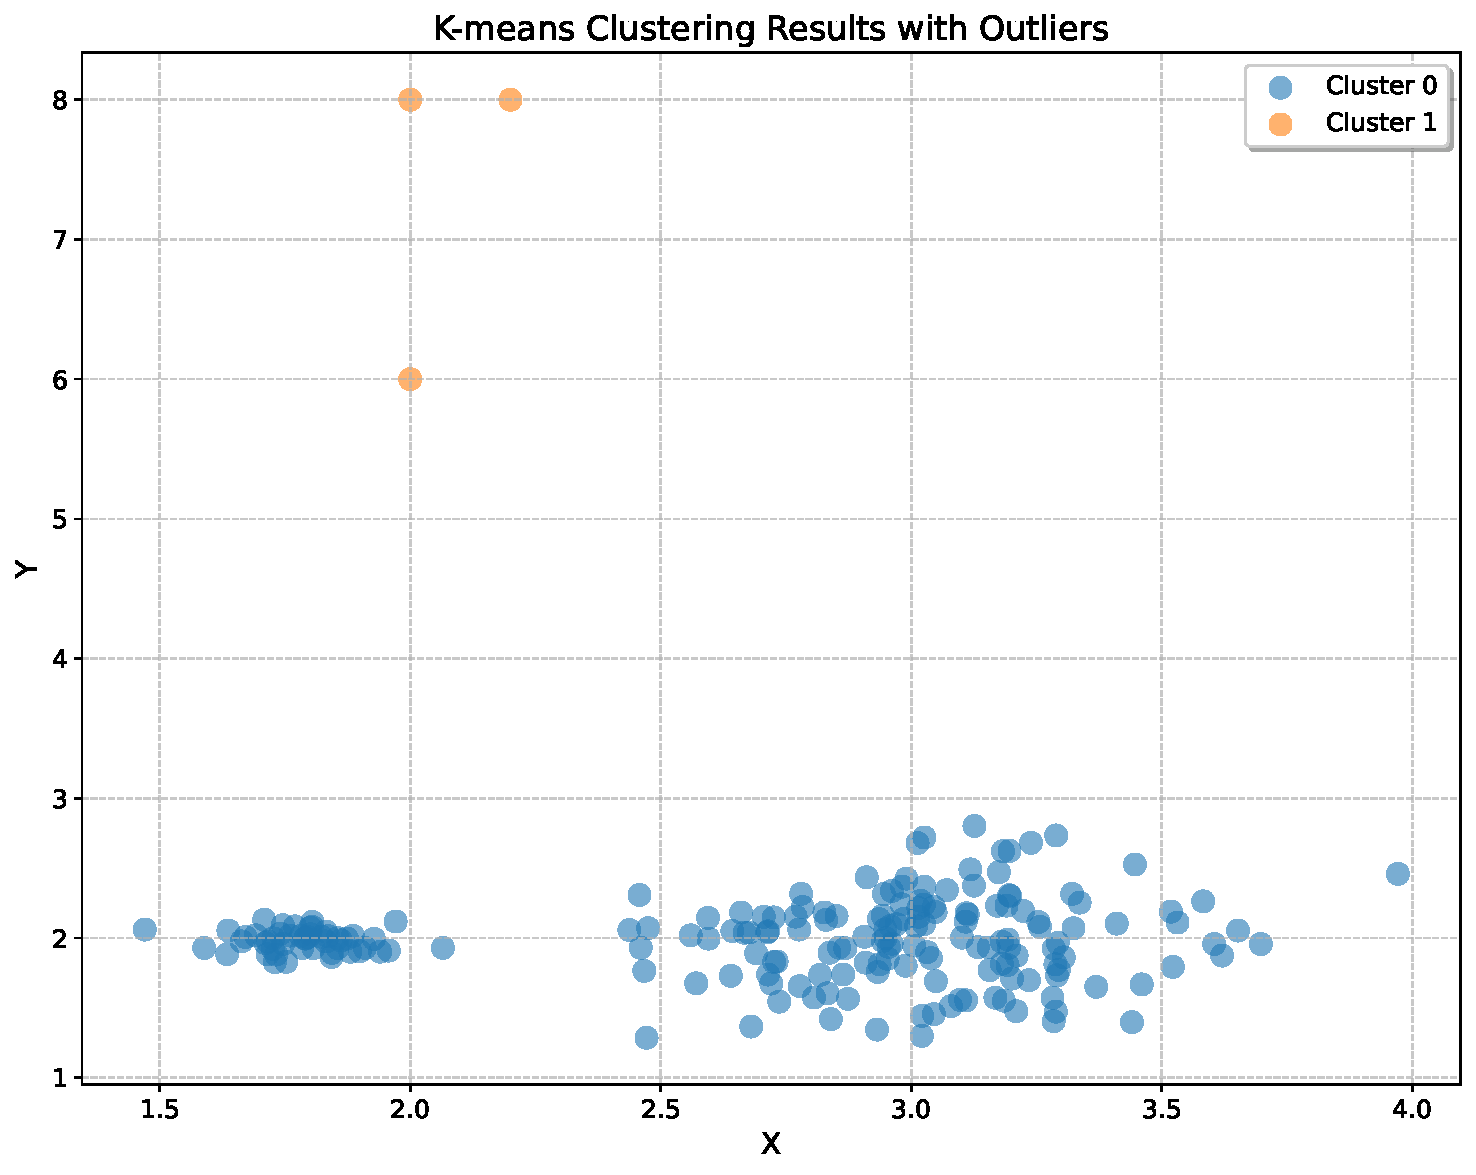
\includegraphics[width=.4\textwidth]{two_island_with_outlier_output_plot_special.pdf}
  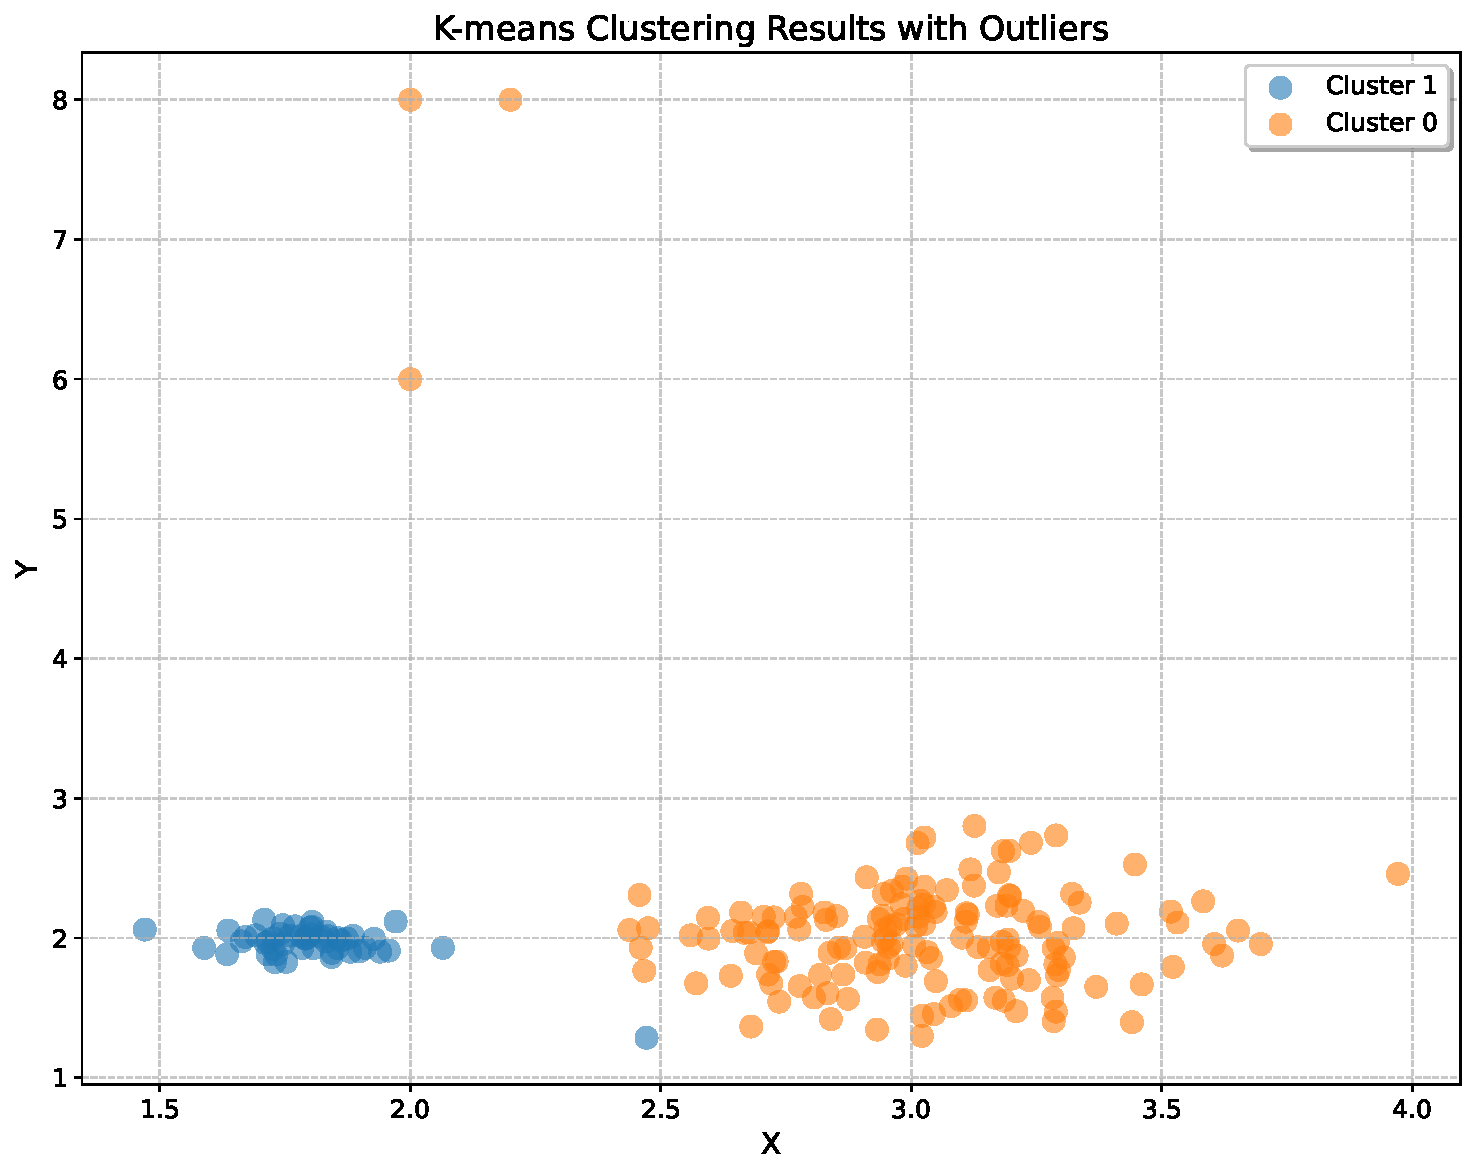
\includegraphics[width=.4\textwidth]{two_island_with_outlier_output_plot.pdf}
  \caption{外れ値を除外しない場合の \texttt{two\_island} クラスタリング例(2 パターン)}
  \label{fig:two-island-with-outlier}
\end{figure}

一方,外れ値を除外してからクラスタリングした結果を図~\ref{fig:two-island-with-outlier_right} に示す。こちらでは 2 島構造が正確に分離されており,LOF による前処理の有効性が視覚的に確認できる。

\begin{figure}[H]
  \centering
  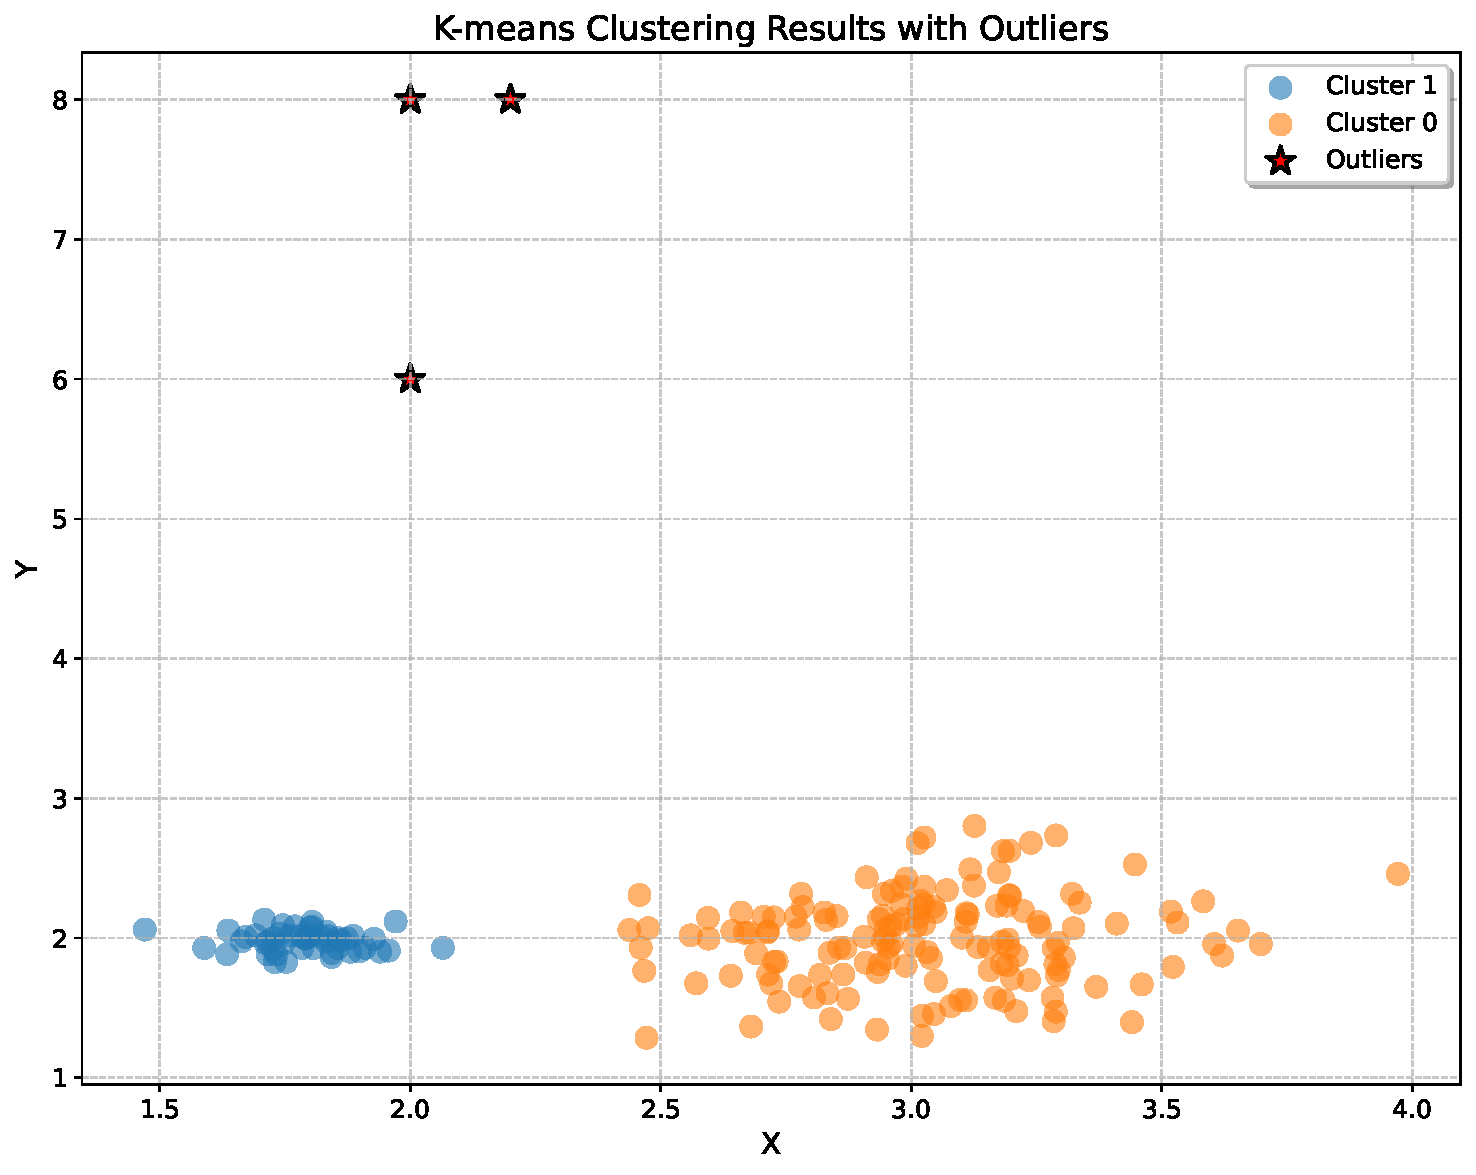
\includegraphics[width=.4\textwidth]{two_island_with_outlier_output_plot_right.pdf}
  \caption{外れ値を除外した場合の \texttt{two\_island} クラスタリング結果}
  \label{fig:two-island-with-outlier_right}
\end{figure}

\subsubsection{結果が分岐した要因}
外れ値を除去しない場合に 2 通りの結果が生じたのは,初期重心が外れ値に設定されるか否かによる。ログを解析したところ,外れ値 3 点のいずれかが初期重心に選ばれたケースでは誤った分割が生じることが判明した。

\subsection{k-means の性質と適用範囲}
\subsubsection{k-means が適する場合}
境界がほぼ直線的なデータ(例:\texttt{square})では,k-means は高速かつ高精度にクラスタを分割できる。実装が簡易で計算コストも低いため,大規模データにおいて依然有力な選択肢である。

\subsubsection{k-means が苦手な場合}
曲線状に点が分布するデータ(例:\texttt{moon},\texttt{crater})では精度が低下する。重心計算がユークリッド距離の平均に依存し,曲線をまたぐ点が同一クラスタに取り込まれるためである。

\subsubsection{手法選択の指針}
\begin{itemize}
  \item \textbf{形状が単純で直感的}: k-means を優先。
  \item \textbf{形状が複雑または非線形}: DBSCAN など密度ベース手法を検討。
  \item 外れ値が多い場合は,どの手法でも LOF などで事前に除去すると結果が安定する。
\end{itemize}

\subsection{今後の改善点}
曲線形状への対策として k-means++ による初期値改良や,ユークリッド以外の距離関数の採用が考えられる。また,DBSCAN と k-means を組み合わせたハイブリッド手法の検討も一案である。

%--------------------------------------------------
\section{まとめ}
本稿で示した C\# プログラムは,LOF による外れ値検出と k-means クラスタリングを連続実行し,200 点のデータに対して 13 反復で収束した。外れ値除去付き重心計算(配列 \texttt{centroid[j,*]})がクラスタ分割の安定化に寄与することを確認した。

今後の課題として,LOF 閾値の最適化,自動初期化手法(k-means++),および非線形クラスタリング手法(DBSCAN)の比較実装を挙げる。

\end{document}

